% !TEX root = ../../ozan_sener_thesis.tex
\section{Why do we need robot knowledge bases?}
Over the last decade, we have seen many successful applications of large-scale knowledge systems.
%  many inclusive web services have been developed  by successfully combining information at a large-scale.
Examples include  Google knowledge graph \cite{dong2014knowledge}, IBM Watson~\cite{ferrucci2010}, Wikipedia,
 and many others.
These systems know answers to many of our day-to-day questions, and
 not crafted for a specific task, which makes them valuable for humans.
Inspired by them, researchers have aggregated domain specific knowledge by mining
data~\cite{dbpedia2007, freebase2008}, and processing natural
language~\cite{nell2010}, images~\cite{imagenet2009} and
speech~\citep{mohamed2011deep}.  These sources of knowledge are specifically designed for humans, and their  human centric design makes them of limited use for robots---for example, imagine a robot querying a search engine
 for how to ``bring sweet tea from the kitchen" (Figure~\ref{fig:intro}).


 %Contrary to humans, for whom incomplete and ambiguous instructions may suffice,
 In order to perform a task, robots require access to a large variety of information with finer details for performing
 perception, planning, control and natural language understanding. When asked to bring sweet tea, as shown in Figure~\ref{fig:intro}, the robot
 would need access to the knowledge for grounding the language symbols into physical entities,
  the knowledge that sweet tea can either be on a table or in a fridge, and the knowledge for inferring the
 appropriate plans for grasping and manipulating objects. Efficiently handling this joint knowledge representation across different
 tasks and modalities is still an open problem.

In this chapter we present \robobrain{} that allows robots to learn and share such representations of knowledge.
We learn these knowledge representations from a variety of sources, including interactions that robots have while performing perception,
planning and control, as well as natural language and visual data from the Internet.
Our representation considers several modalities including symbols, natural language, visual or shape features, haptic properties, and so on. \robobrain{} connects this knowledge from various sources and allow robots to perform diverse tasks by jointly reasoning over multiple data modalities.  %Moreover, our experiments suggest that by connecting different modalities and projects, robots can share knowledge and collectively improve their abilities.

 \begin{figure}
 \centering
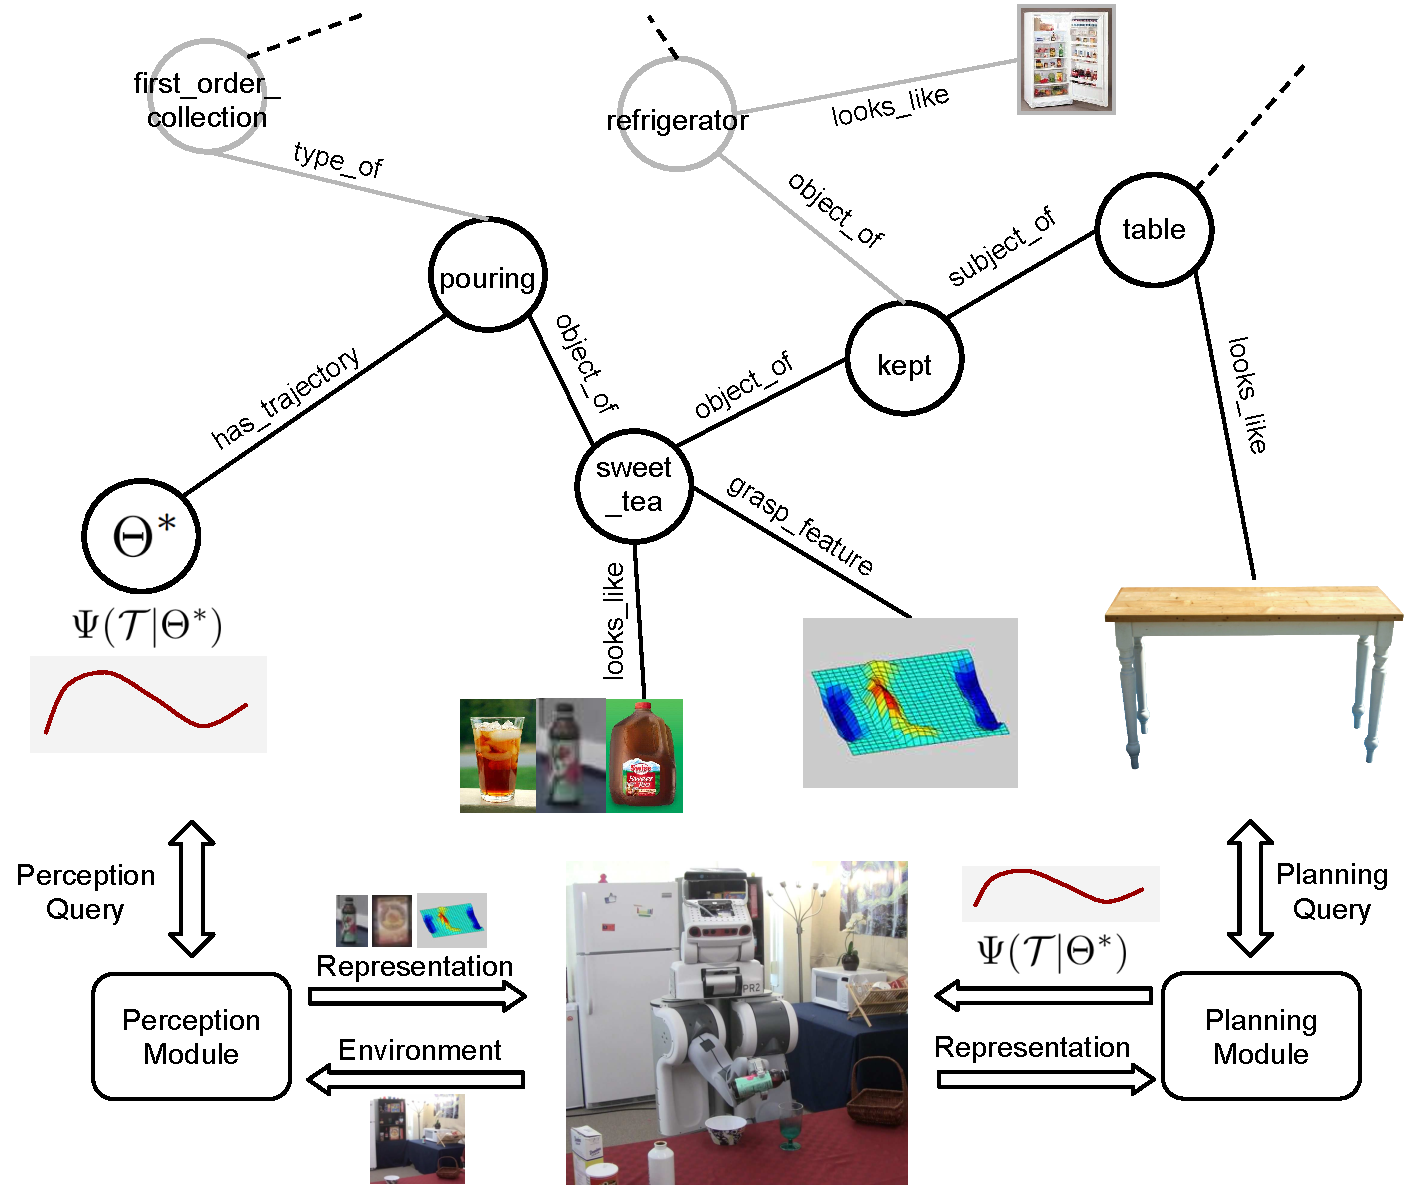
\includegraphics[width=\linewidth]{Image/cover_picture_graph}
 \caption{\textbf{An example showing a robot using \robobrain{} for performing tasks.}  The robot is asked ``Bring me sweet tea from the kitchen", where
 it needs to translate the instruction into the perceived state of the environment.
\robobrain{} provides useful knowledge to the robot for performing the task:
 (a) sweet tea can be kept on a table or inside a refrigerator,
 (b) bottle can be grasped in certain ways,
 (c) opened sweet tea bottle needs to be kept upright,
 (d) the pouring trajectory should obey user preferences of moving slowly to pour, and
 so on.
 }
 \label{fig:intro}
 \end{figure}

\begin{figure*}[t]
\centering
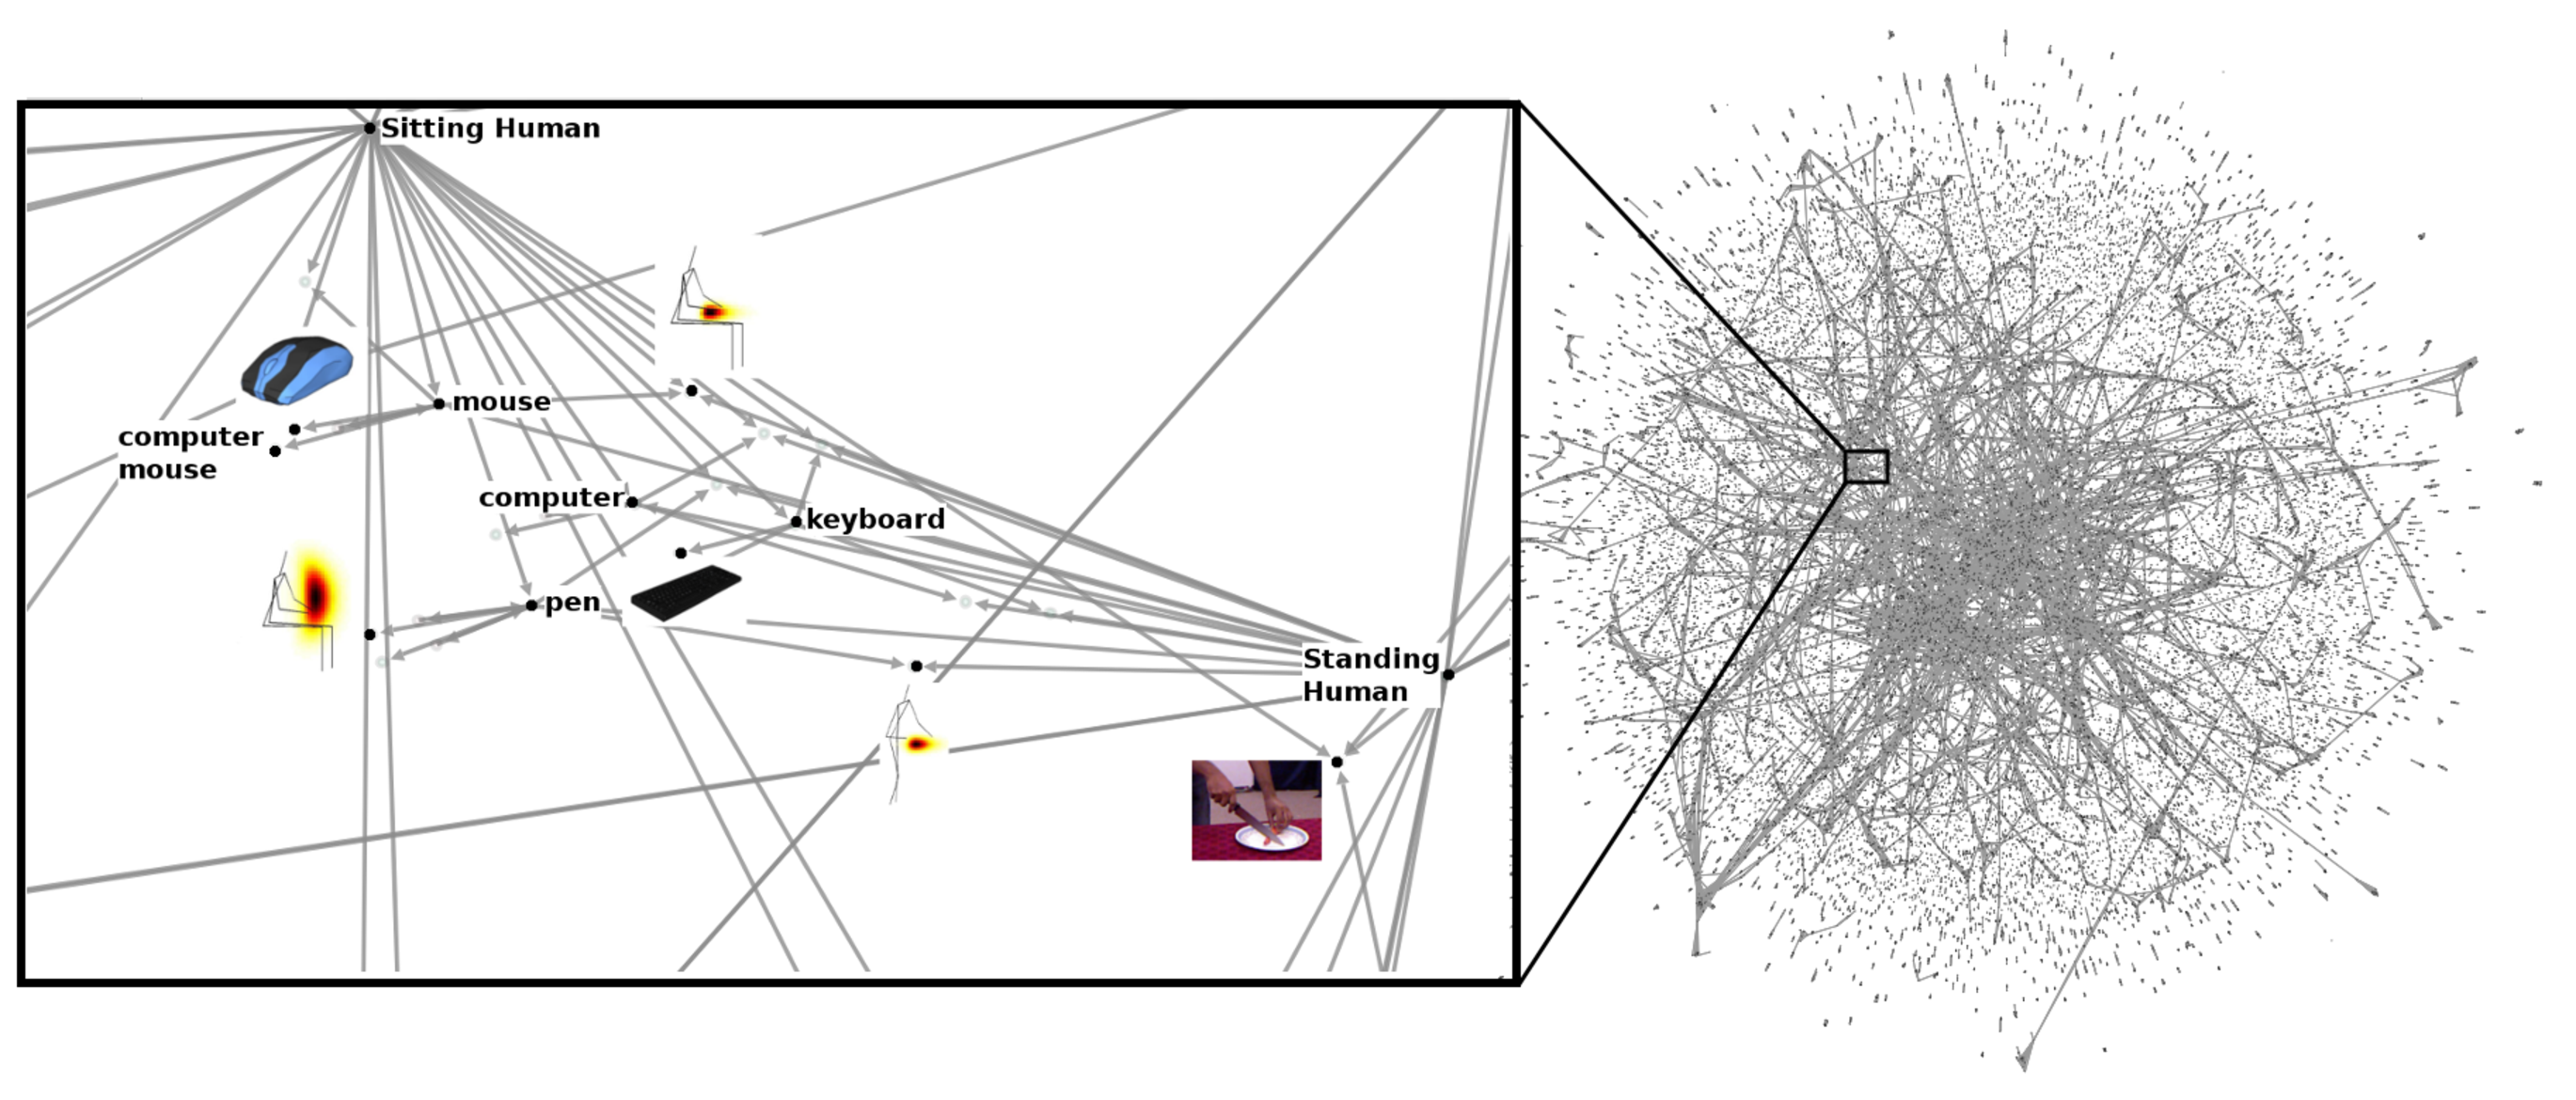
\includegraphics[width=.95\linewidth, height=2.6in, clip=true, trim=0 40 0 0]{Image/RBgraph}
\caption{\textbf{A visualization of the \robobrain{} graph} on Nov 2014, showing about 45K nodes and 100K directed edges.
%  from the RoboBrain's knowledge graph.
The left inset shows a zoomed-in view of a small region of the graph with rendered media. This illustrates the relations between multiple modalities namely images, heatmaps, words and human poses. \textit{For high-definition graph visualization, see: \url{https://sites.google.com/site/robotknowledgeengine/}}}
\label{fig:graph}
\end{figure*}


\robobrain{} enables sharing from multiple sources by representing the knowledge in a graph structure.
% RKE enables knowledge sharing by representing the knowledge in a graph representation.
% Thcontaining
% out of the
% information that robots need for performing various tasks.
%Knowledge in  RKE comes from multiple sources, which is integrated into the graph structure of RKE.
Traversals on the \robobrain{} graph allow robots to gather the specific information they need for a task. This includes the  semantic information, such as different grasps of the same object, as well as the functional knowledge, such as spatial constraints (e.g., a bottle is kept on the table and not the other way around).
The key challenge lies in building this graph from a variety of knowledge sources while ensuring dense connectivity across nodes. Furthermore, there are several  challenges in building a system that allows concurrent and distributed update, and retrieval operations.

We  present use of \robobrain{} on three robotics applications in the area of grounding natural language, perception and planning.
For each application we show usage of \robobrain{} \textit{as-a-service}, which allow researchers to effortlessly use the state-of-the-art algorithms. We also present experiments to show that sharing knowledge representations through \robobrain{} improves existing language grounding and path planning algorithms.


\robobrain{} is a collaborative project that we support by designing a large-scale cloud architecture.
%and we designed a large-scaled cloud architecture to enable this collaboration efficiently.
In the current state, \robobrain{} stores and shares knowledge across several research projects~\cite{tellex2011understanding,misra2014tell,jainsaxena2013_trajectorypreferences,jiang-hallucinatinghumans-labeling3dscenes-cvpr2013,jiang2012humancontext,KoppulaRSS2013,wulenzsaxena2014_hierarchicalrgbdlabeling,lenz2013_deeplearning_roboticgrasp} and Internet knowledge sources~\citep{cyc1995,wordnet1998}.
% RKE has knowledge from \cite{misra2014tell,tellex2011understanding,jainsaxena2013_trajectorypreferences,jiang-hallucinatinghumans-labeling3dscenes-cvpr2013}.
We believe as more research projects contribute knowledge to \robobrain{}, it will not only improve the concerned project but will
also be beneficial for the robotics community at large.
%their robots perform better but we also believe this will be beneficial for the robotics community at large.
%The RKE is under open Creative Commons Attribution license\footnote{http://creativecommons.org/licenses/by/2.5, Extra conditions may apply depending on the data sources, see anonymous.me for detailed information.} and is
%avalable at: \texttt{\url{http://anonymous}}

The goal of the chapter is to present an overall view of the \robobrain{}, its architecture, functionalities, and demonstrate its application to robotics. In Section~\ref{sec:graph} we formally define the \robobrain{} graph and describe its
system architecture in Section~\ref{sec:system}. In order for robots to use
\robobrain{} we propose the Robot Query Library in Section~\ref{sec:raquel}. In
Section~\ref{sec:applications} we present different robotic applications using \robobrain{}.
